The MIMO radar has attracted the attention of researchers in the last decades, because of its
advantages over standard phase-array radar in terms of \cite{stoica2007probing}:
\begin{enumerate}
    \item adaptive localization and detection techniques;
    \item freely-chosen probing signal that can approximate a desired beampattern and minimize the cross-correlation.
\end{enumerate}

A MIMO radar system model is shown in Fig.\ref{fig:mimo-radar-system-model}. 
If the transmitter and receiver in radar
system share the same hardware, it is mono-static radar, while it is classified as bi-static radar if they are separated.

\begin{figure}[htbp]
    \centering
    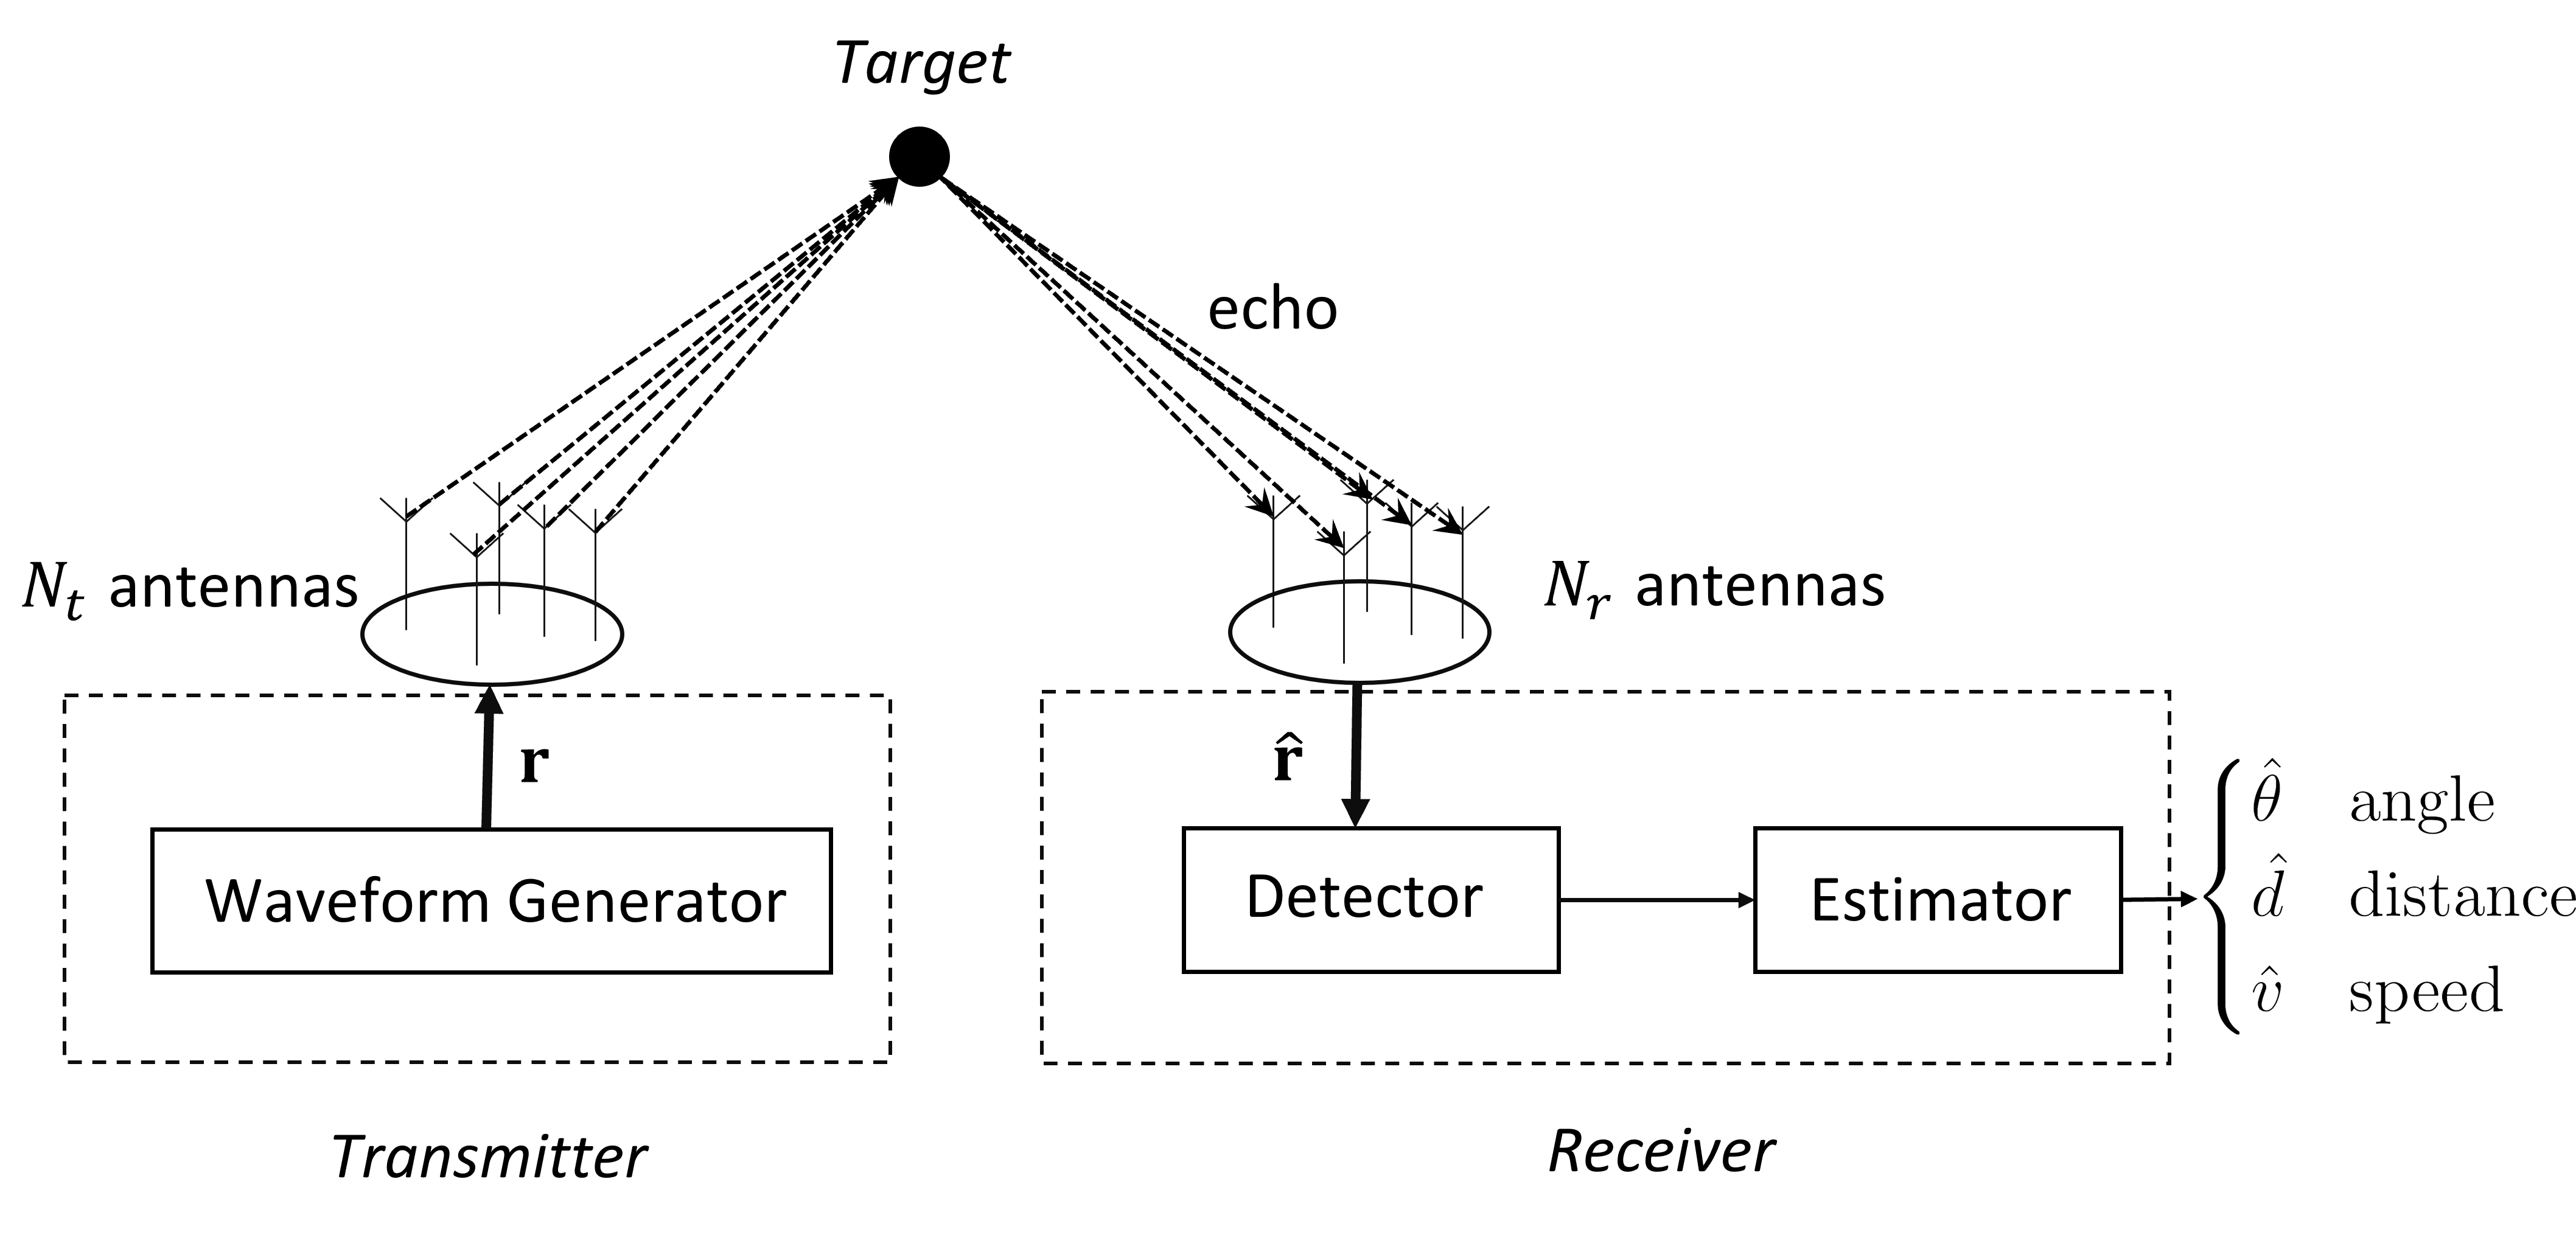
\includegraphics[width=1.0\textwidth]{./mimo-radar-system.png}
    \caption{MIMO radar system model}
    \label{fig:mimo-radar-system-model}
\end{figure}

\subsection{Radar Waveform Design}
The radar waveform ${\bf r}$ generated by the waveform generator should satisfy some radar-specific shaping constraints \cite{liu2020tutorial}:
\begin{enumerate}
    \item \textit{Low Sidelobe Level}: This is to reduce the interference from undesired directions. Generally, the probing power
    at target locations is maximized or the desired beampattern is achieved to satisfy this constraint.
    \item \textit{Low Peak-to-Average Power Ratio}: A radar system generally transmits signals at the maximum power budget to ensure
    the SNR of the echo signal is enough for detector. For the high power radar, the low peak-to-average power ratio is preferred to reduce 
    to signal distortion. The optimal method is to use a constant-modulus waveform, i.e., the power fed to each antenna is the same.
    \item \textit{Clutter Suppression}: When there are multiple targets, the clutter interference is generated from undesired targets.
    In this case, the waveform should be carefully designed to have small cross-correlation in different target directions \cite{stoica2007probing}.
\end{enumerate}

The MIMO radar waveform can be designed to maximize the probing power in direction $\theta$:
% An example of a probing signal design for a MIMO radar with single known target is:

\begin{subequations}
    \begin{align}
      \max_{{\bf R}} \quad & {\bf a}^H(\theta) {\bf R} {\bf a}(\theta) \\
      \mathrm{s.t.} \quad & \mathrm{diag}({\bf R}) = c{\bf 1}_{N_t}, \\ 
      & {\bf R} \succeq 0,
    \end{align}
\end{subequations}
where ${\bf{a}}(\theta) = [1, e^{j\frac{2\pi}{\lambda}d\sin({\theta})},...,e^{j\frac{2\pi}{\lambda}d(N_t-1)\sin({\theta})}]^T$
is the steering vector in direction of $\theta$ and ${\bf R} = \mathbb{E}({\bf{r}}{\bf{r}}^H)$ is the covariance matrix of radar signal.
In this design, the porbing power ${\bf a}^H(\theta) {\bf R} {\bf a}(\theta)$ is maximized under the constant-modulus constraint 
$\mathrm{diag}({\bf R}) = c{\bf 1}_{N_t}$. More waveform designs for MIMO radar can be found in \cite{stoica2007probing}.

\subsection{Radar Performance Metrics} \label{sec:radar_metric}

There are two main tasks for a radar system: detection and estimation. Detection is to justify whether targets are present or not,
while estimation is to extract target parameters, including angle, distance, and speed, from echo signals.

\subsubsection{Detection}
For detection problem, the binary hypothesis testing is normally applied \cite{liu2020tutorial}
\begin{equation}\label{eqn:hypothesis_testing}
    \hat{\bf r}(t) = \begin{cases} 
        \mathcal{H}_0: & {\bf z}(t),\\
        \mathcal{H}_1: & \beta e^{2j\pi f_D t}{\bf s}_r(\varphi) {\bf s}_t^T(\varphi){\bf r}(t - \tau) + {\bf z}(t).
    \end{cases}
\end{equation}
% where $\mathcal{H}_0$ is the case that radar receives nothing but interference plus noise ${\bf z}(t)$, while $\mathcal{H}_1$ is the case that 
% radar receives both echo and interference plus noise. Specifically, $\beta$ represents for the complex round-trip path loss and radar cross-section effect, 
% $f_D = 2vf_c / c$ is the Doppler frequency, $f_c$ is the carrier frequency, $c$ is the light speed, ${\bf b}(\theta) \in \mathbb{C}^{N_r \times 1}$
% denotes the receive steering vector, ${\bf a}(\theta) \in \mathbb{C}^{N_t \times 1}$ denotes the transmit steering vector, and
% $\tau = 2d / c$ is the round-trip delay. 
There are two conditions in received signal $\hat{\bf r}(t)$: 
\begin{itemize}
    \item $\mathcal{H}_0$: only interference plus noise ${\bf z}(t)$.
    \item $\mathcal{H}_1$: echo signals $\beta e^{2j\pi f_D t}{\bf s}_r(\varphi) {\bf s}_t^T(\varphi){\bf r}(t - \tau)$ and interference plus noise.
\end{itemize}
Specifically, $\beta$ represents for the complex round-trip path loss and radar cross-section effect. $f_D = 2vf_c / c$ is the Doppler frequency. 
where $v$ is the speed of target.
${\bf s}_r(\theta) \in \mathbb{C}^{N_r \times 1}$ and ${\bf s}_t(\theta) \in \mathbb{C}^{N_t \times 1}$ are receive and transmit steering vectors
in direction of $\varphi$.

The final step of hypothesis testing is designing a detector $\mathcal{T}(\cdot)$ and then the output of detector is compared 
with a pre-set threshold $\tau$
\begin{equation} \label{eqn:radar-detection}
    \mathcal{T}(\hat{\bf r}) \underset{\mathcal{H}_1}{\overset{\mathcal{H}_0}{\lessgtr} } \tau.
\end{equation}
The radar performance are mainly evaluated by two metrics:
\begin{enumerate}
    \item Detection probability $P_D$: target is present and detected by the radar.
    \item False-alarm probability $P_{FA}$: target is not present but detected by the radar.
\end{enumerate}

However, $P_D$ and $P_{FA}$ are usually complicated and not easy to be optimized. For this problem, a method is to relax 
them to a simple metric, which is shown in the following example.

Generalized likelihood ratio test (GLRT) is a popular method in detector. The detection probability in GLRT that determined by the 
Neyman-Pearson criterion is given as \cite{wang2020ris}:
\begin{equation}
    P_D = 1 - \mathfrak{F}_{\mathcal{X}_2^2(\rho)}\Big(\mathfrak{F}_{\mathcal{X}_2^2}^{-1}(1-P_{FA})\Big),
\end{equation}
where $\mathfrak{F}_{\mathcal{X}_2^2(\rho)}$ is the non-central chi-square cumulative distribution function (CDF), and 
$\mathfrak{F}_{\mathcal{X}_2^2}^{-1}$ denotes the inverse operation. If the orthogonal radar signal is used, i.e., ${\bf R_r} = \mathbb{E}({\bf rr}^H) = P_R {\bf I}_{N_t}$,
the parameter $\rho$ is given as \cite{wang2020ris}:
\begin{equation}
    \rho = |\beta|^2 P_R {\rm Tr}\Big( {\bf CC}^H {\bf R}_{\bf z}^{-1} \Big),
\end{equation}
where ${\bf C} = {\bf s}_r(\theta) {\bf s}_t^T(\theta)$ and ${\bf R}_{\bf z} = \mathbb{E}({\bf zz}^H)$ is the covariance matrix of noise plus interference. The maximization problem of $P_D$ can be converted to 
the maximization problem of $\rho$, because $P_D$ is monotonically increasing with $\rho$. As the covariance matrix ${\bf R}_{\bf z}$
is positive semidefinite, we have
\begin{align}
    {\rm Tr}&\Big( {\bf CC}^H {\bf R}_{\bf z}^{-1}{\bf R}_{\bf z} \Big) \leq {\rm Tr} \Big( {\bf CC}^H {\bf R}_{\bf z}^{-1} \Big) {\rm Tr}({\bf R}_{\bf z})\\
    \Rightarrow \rho &= |\beta|^2 P_R {\rm Tr} \Big( {\bf CC}^H {\bf R}_{\bf z}^{-1} \Big) \nonumber\\
    &\geq \frac{|\beta|^2 P_R{\rm Tr}\Big( {\bf CC}^H \Big)}{{\rm Tr}({\bf R}_{\bf z})}  \nonumber\\
    &= \frac{|\beta|^2 {\rm Tr}\Big( {\bf C}{\bf R_r} {\bf C}^H \Big)}{{\rm Tr}({\bf R}_{\bf z})} \nonumber \\
    &= \text{SINR}_{\text{echo}}
\end{align}
The parameter $\rho$ is lower bounded by the SINR of the echo signal. Thus, the maximization problem of detection probability
can be relaxed to the maximization problem of SINR of the echo signal.


\subsubsection{Estimation}
Once the target is detected, the target parameters, i.e., angle, distance, and speed, are extracted from ${\bf y}(t)$ by an 
estimator $\mathcal{F}(\cdot)$:
\begin{equation}
    \mathcal{F}(\hat{\bf r}) = \{ \hat{\theta}, \hat{d}, \hat{v} \}.
\end{equation}
The estimator for each parameter is normally designed separately. For example, the angle can be estimated using subspace methods like
MUltiple SIgnal Classification (MUSIC) \cite{schmidt1986multiple}. The distance and speed can be estimated using matched-filtering 
algorithm \cite{liu2020road}.

Mean square error (MSE) between estimated and true values is an important metric to measure the estimator performance.
However, the Cramér-Rao lower bound is normally used in practice because a closed-form MSE is difficult to derive.
